\begin{appendix}
\section{Distribution of Audio Features}
\label{appendix:A}
We plotted the individual distributions of the original 13 audio features (a) and those features after normalisation (b) to check for any correlations between them
\begin{figure}[H]
\begin{subfigure}{1\textwidth}
\centering
    \includegraphics[scale=0.2]{Outputs/Boxplot - Original Audio Features.png}
    \captionsetup{justification=centering,margin=1cm}
    \caption{Boxplot of original audio features as retrieved from the Spotify API}
    \label{fig:sub-first}
\end{subfigure}
\newline
\begin{subfigure}{1\textwidth}
\centering
    \includegraphics[scale=0.3]{Outputs/Boxplot - Normalised Audio Features.png}
    \captionsetup{justification=centering,margin=1cm}
    \caption{Boxplot of normalised audio features}
    \label{fig:sub-second}
\end{subfigure}
\end{figure}

\section{Dimensionality Reduction}
\label{appendix:B}
\subsection{PCA}
\begin{figure}[h!]
\centering
\centerline{\includegraphics[scale=0.3]{Outputs/PCA - Number of Components.png}}
\captionsetup{justification=centering,margin=1cm}
\caption{Cumulative explained variance of PCA on the original dataset with 13 features. 7 components yield 95\% of the variance}
\end{figure}

\subsection{Grid Search for UMAP with K-Means}
Grid Search is an exhaustive hyperparameter tuning technique that helps in determining the optimal values of parameter combinations for a model. We created a pipeline to find the optimal number of clusters for K-Means with UMAP reduced audio features.

\newlength\dunder
\settowidth{\dunder}{\_}
The following parameters were used
\begin{table}
\begin{center}
\resizebox{\columnwidth}{!}{%
\begin{tabular}{cc|c|c|c|c|c}
\multicolumn{2}{c}{} & \multicolumn{5}{c}{} \\ \cline{3-6}
\multicolumn{2}{c|}{} & \texttt{umap\rule{2\dunder}{0.02pt}n\rule{1\dunder}{0.1pt}neighbors} &
\texttt{umap\rule{2\dunder}{0.02pt}min\rule{1\dunder}{0.1pt}dist} &
\texttt{umap\rule{2\dunder}{0.02pt}n\rule{1\dunder}{0.1pt}components} &
\texttt{kmeans\rule{2\dunder}{0.02pt}n\rule{1\dunder}{0.1pt}clusters} \\ \cline{3-6}
&&5&0.1&2&2& \\ \cline{3-6}
&&10&0.4&3&7& \\ \cline{3-6}
&&20&0.6&-&15& \\ \cline{3-6}
&&50&0.9&-&20& \\ \cline{3-6}
&&100&-&-&30& \\ \cline{3-6}
&&-&-&-&50& \\ \cline{3-6}
\end{tabular}%
}
\end{center}
\caption{Grid Search parameters for UMAP with K-Means}
\end{table}

The best parameters returned by the search were kmeans\rule{2\dunder}{0.02pt}n\rule{1\dunder}{0.1pt}clusters: 50, umap\rule{2\dunder}{0.02pt}min\rule{1\dunder}{0.1pt}dist: 0.1, umap\rule{2\dunder}{0.02pt}n\rule{1\dunder}{0.1pt}components: 2, umap\rule{2\dunder}{0.02pt}n\rule{1\dunder}{0.1pt}neighbors: 100

And the clustering results were as follows
\begin{figure}[h]
    \centering
    \includegraphics[scale=0.07]{Outputs/Cluestering - UMAP Grid Search Features.png}
    \caption{K-Means with UMAP derived features after Grid Search}
    \captionsetup{justification=centering,margin=1cm}
    \label{fig:kmeans-umap-gs}
\end{figure}

However, we chose not to go with the search results since 50 clusters are too fine-grained. Hence, we chose the number of clusters returned by the elbow curve.

\subsection{Silhouette Analysis for K-Means}
The success of the the K-Means clustering methods relies on an appropriately selected \textit{k} value or the number of clusters \textit{n\_clusters} to be formed. This number and the other parameters were empirically derived using heuristic methods including elbow plots as shown in the main section of the report above and silhouette analysis.

We experimented with K-Means \textit{n\_clusters} ranging from [2,50] and plotted the corresponding silhouette scores for clustering on features derived by each of the dimensionality reduction algorithms covered above. The optimal number of clusters for K-Means was found to be 2 or 3 based on the results from the majority of the methods. This measure didn't seem appropriate for this task because there weren't enough clusters to adequately capture the variation in the types of songs. Instead, this rating was used as an evaluation tool to contrast the different dimensionality reduction and clustering methods. Due to space constraints, the screenshots of the silhouette plots are not included here. However they can be found in the output cells of our code file \textit{'Spotify Data Analysis.ipynb'}

\subsection{Grid Search - DBSCAN}
We created our own grid search for the DBSCAN algorithm with the following parameters - $eps = [0.1, 0.2, 0.6, 0.8]$ and $min\_samples = [2, 4, 6, 8]$ and reported the Calinski Harabasz score, Davies Bouldin index, Silhouette scores and number of clusters for each combination. We chose the values for \textit{eps} and \textit{min\_samples} that gave us a moderate number of clusters (not too coarse or fine grained), and a good trade-off between the other metrics.
The best set of parameters for each of the dimensionality reductions methods used are reported as follows

\begin{table}
\begin{center}
\begin{tabular}{c|c|c|c|ccc}
\multicolumn{2}{c}{} & \multicolumn{5}{c}{} \\ \cline{3-4}
\multicolumn{2}{c|}{} & \texttt{eps} & \texttt{min\_samples} & \\ \cline{2-4}
& \texttt{Original Audio Features} & 0.6 & 2 & & & \\ \cline{2-4}
 & \texttt{PCA} & 0.2 & 8 & & & \\ \cline{2-4}
& \texttt{UMAP} & 0.2 & 8 & & & \\ \cline{2-4}
& \texttt{Gaussian Random Projections} & 0.2 & 2 & & & \\ \cline{2-4}
& \texttt{PaCMAP}  & 0.8 & 8 & & & \\ \cline{2-4}
& \texttt{Autoencoders}  & 0.6 & 2 & & & \\ \cline{2-4}
\end{tabular}
\end{center}
\caption{Grid Search best parameters for each dimensionality reduction method with DBSCAN}
\end{table}

\section{Clustering Results}
\label{appendix:C}
\subsection{K-Means}
\begin{figure}[h]
    \centering
    \includegraphics[scale=0.08]{Outputs/K-Means Clustering - Original Audio Features.png}
    \caption{K-Means clustering on the scaled original audio features}
    \label{fig:kmeans-first}
\end{figure}
\begin{figure}[!htb]
    \centering
    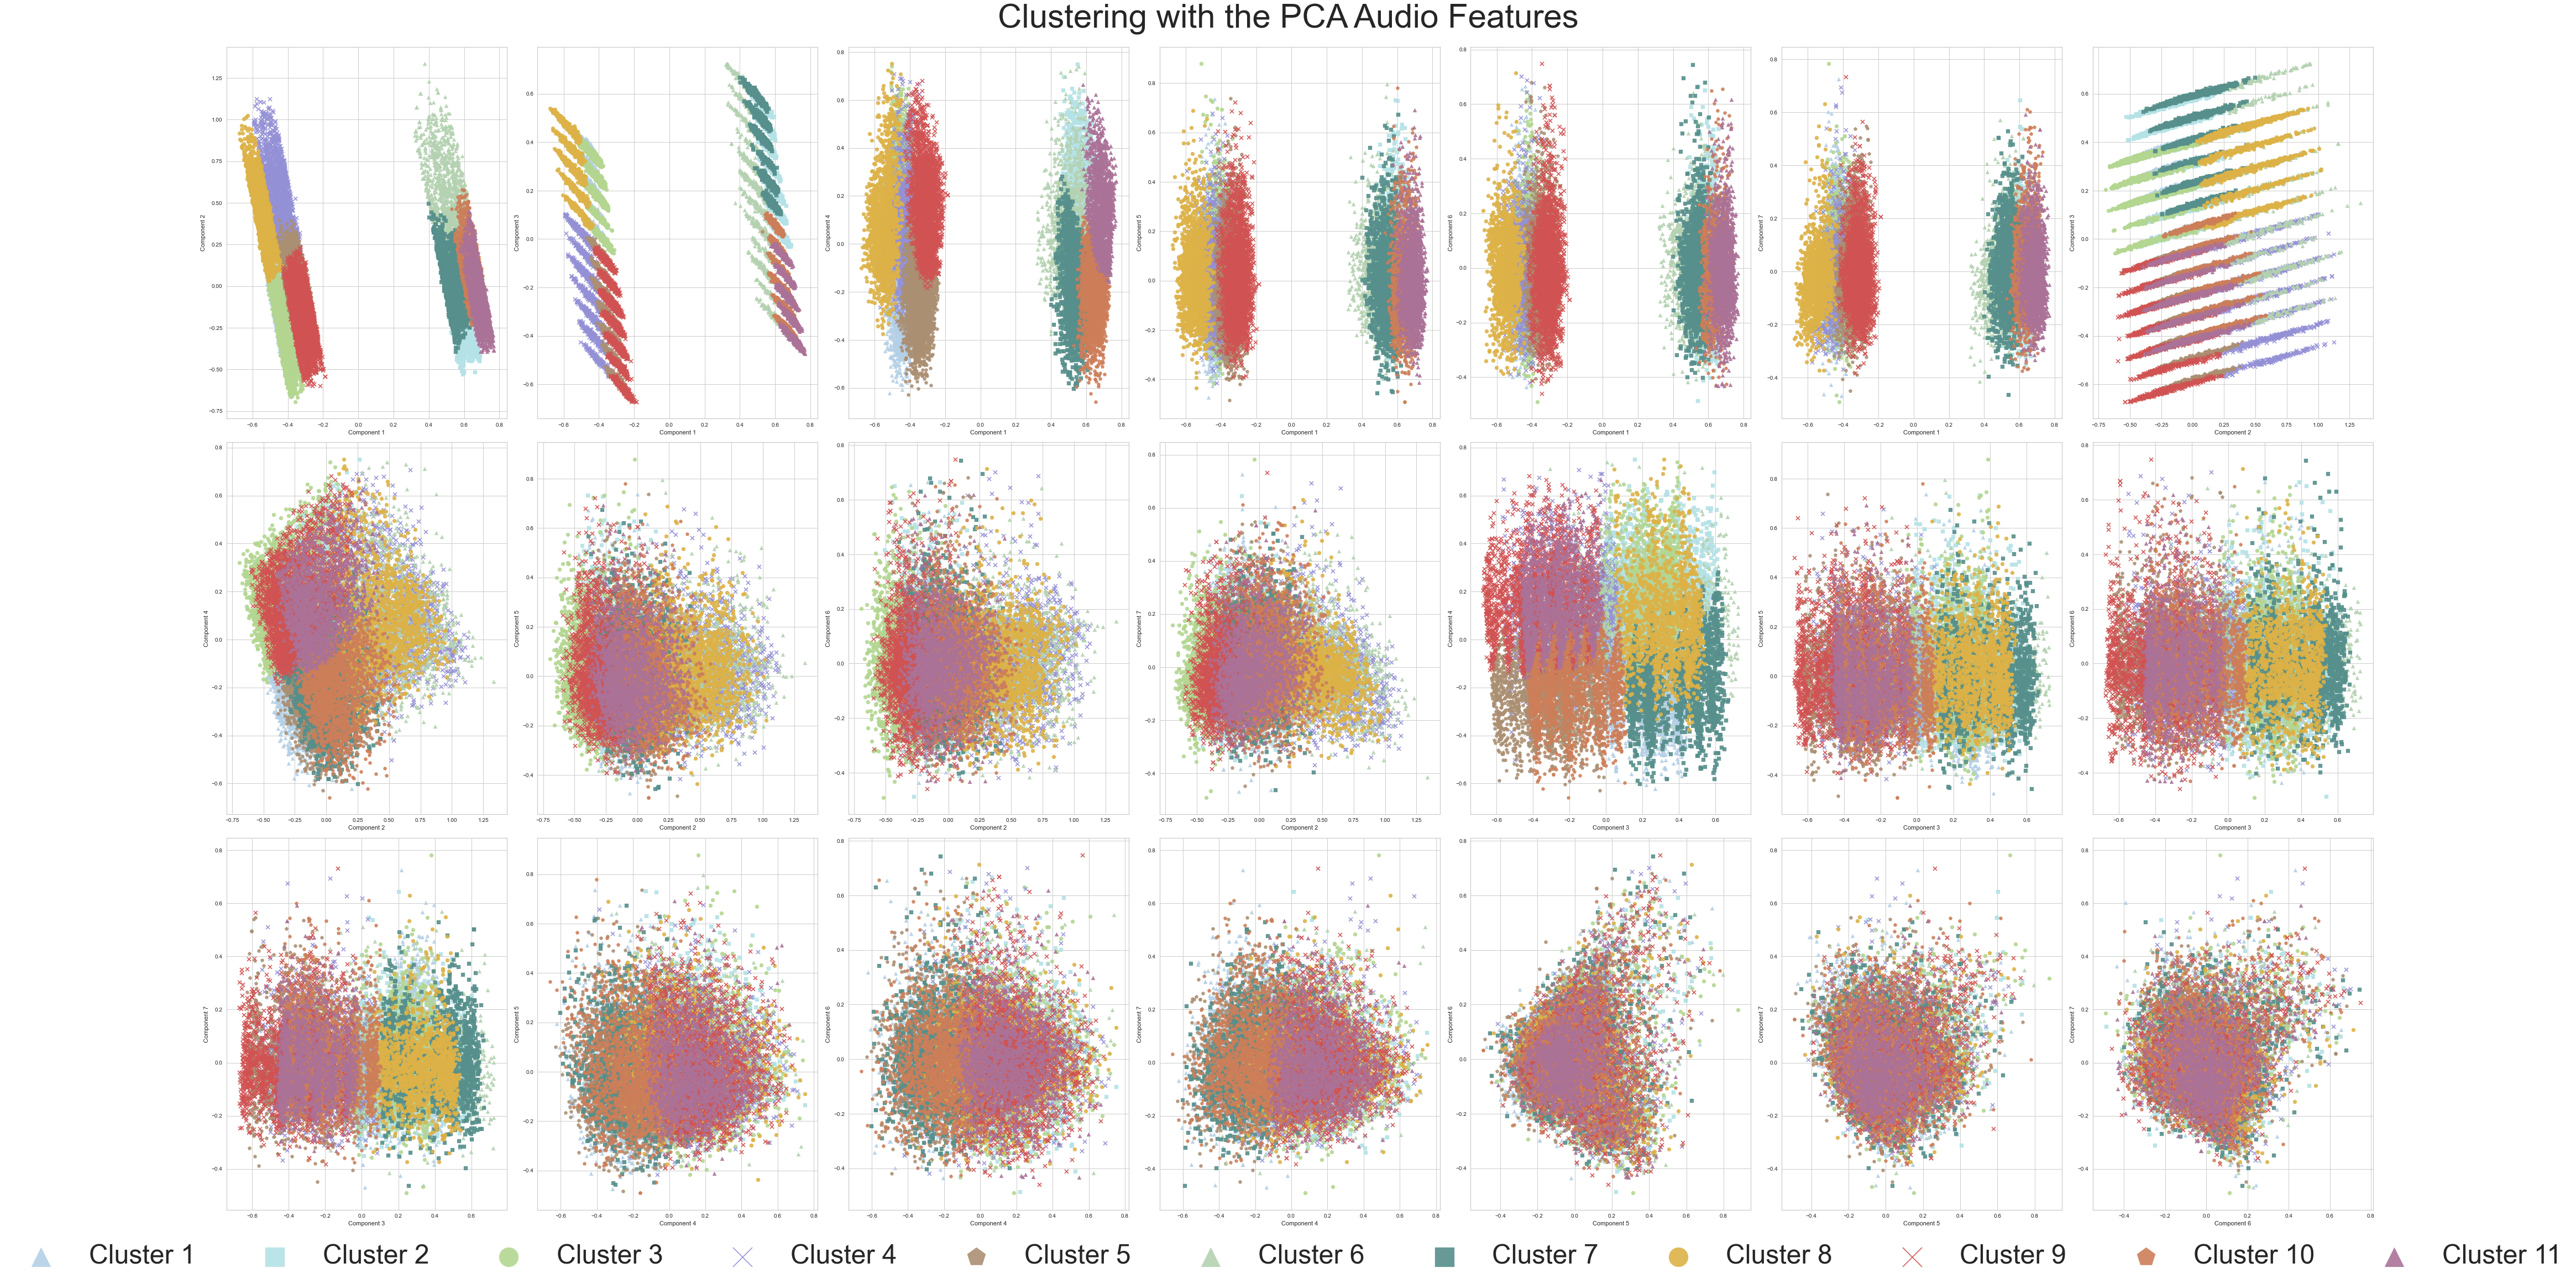
\includegraphics[scale=0.08]{Outputs/K-Means Clustering - PCA Audio Features.png}
    \caption{K-Means clustering on PCA dervived audio features}
    \label{fig:kmeans-second}
\end{figure}
\begin{figure}[!htb]
    \centering
    \includegraphics[scale=0.08]{Outputs/K-Means Clustering - UMAP Audio Features.png}
    \caption{K-Means clustering on UMAP derived audio features}
    \label{fig:kmeans-third}
\end{figure}
\begin{figure}[!htb]
    \centering
    \includegraphics[scale=0.08]{Outputs/K-Means Clustering - Gaussian Random Projections Audio Features.png}
    \caption{K-Means clustering on Gaussian Random Projections derived audio features}
    \label{fig:kmeans-fourth}
\end{figure}
\begin{figure}[!htb]
    \centering
    \includegraphics[scale=0.08]{Outputs/K-Means Clustering - PaCMAP Features.png}
    \caption{K-Means clustering on the PaCMAP derived audio features}
    \label{fig:kmeans-fifth}
\end{figure}
\begin{figure}[!htb]
    \centering
    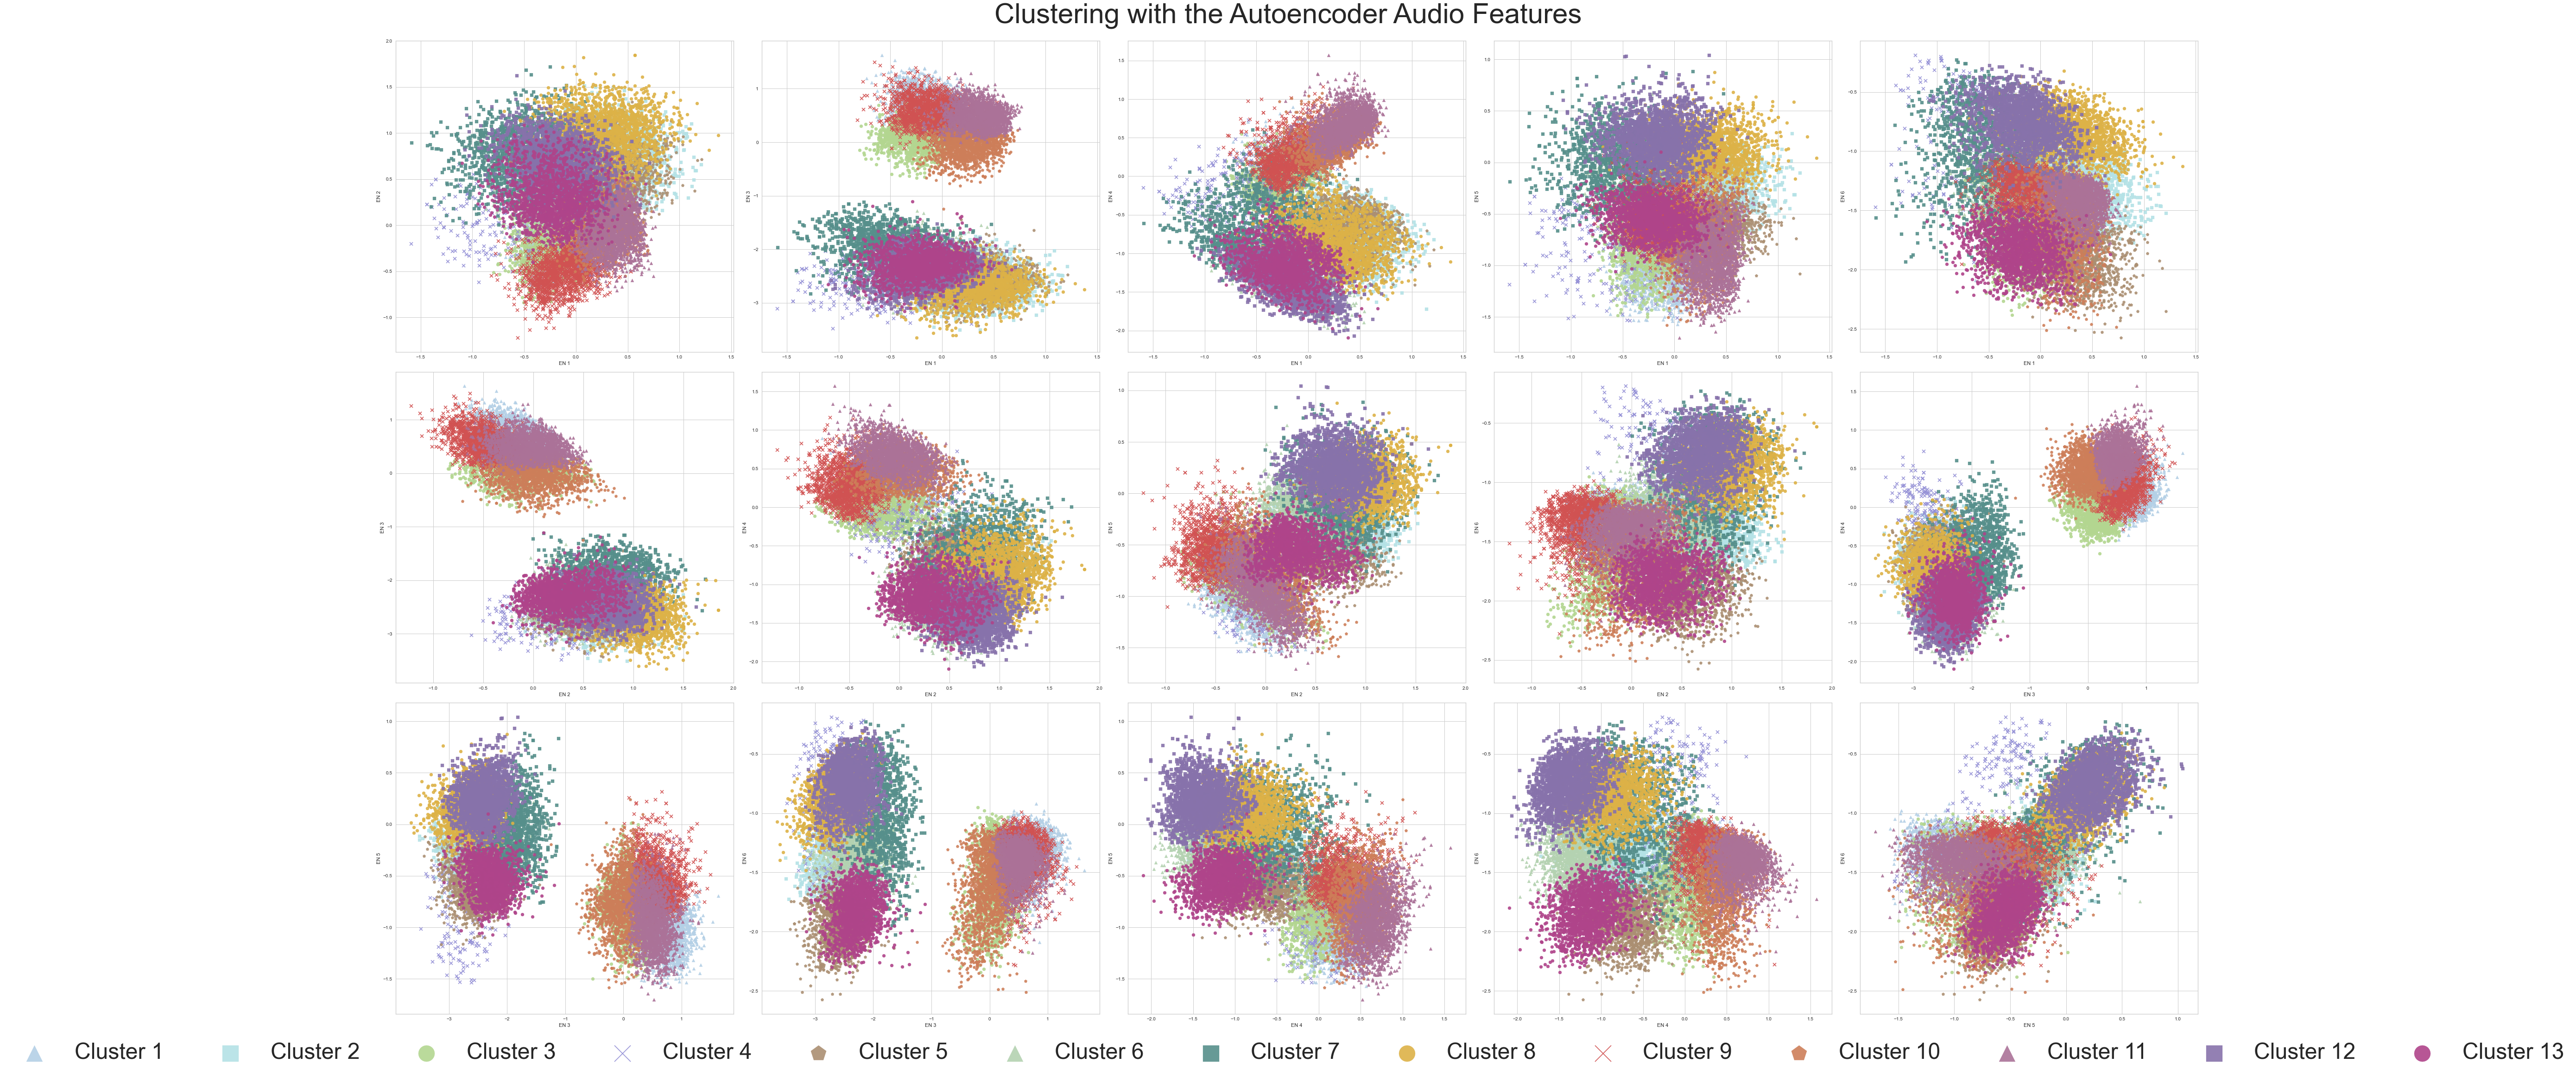
\includegraphics[scale=0.07]{Outputs/K-Means Clustering - Autoencoder Audio Features.png}
    \caption{K-Means clustering on the Autoencoder derived audio features}
    \label{fig:kmeans-sixth}
\end{figure}
\FloatBarrier
\subsection{BIRCH}
\begin{figure}[!htb]
    \centering
    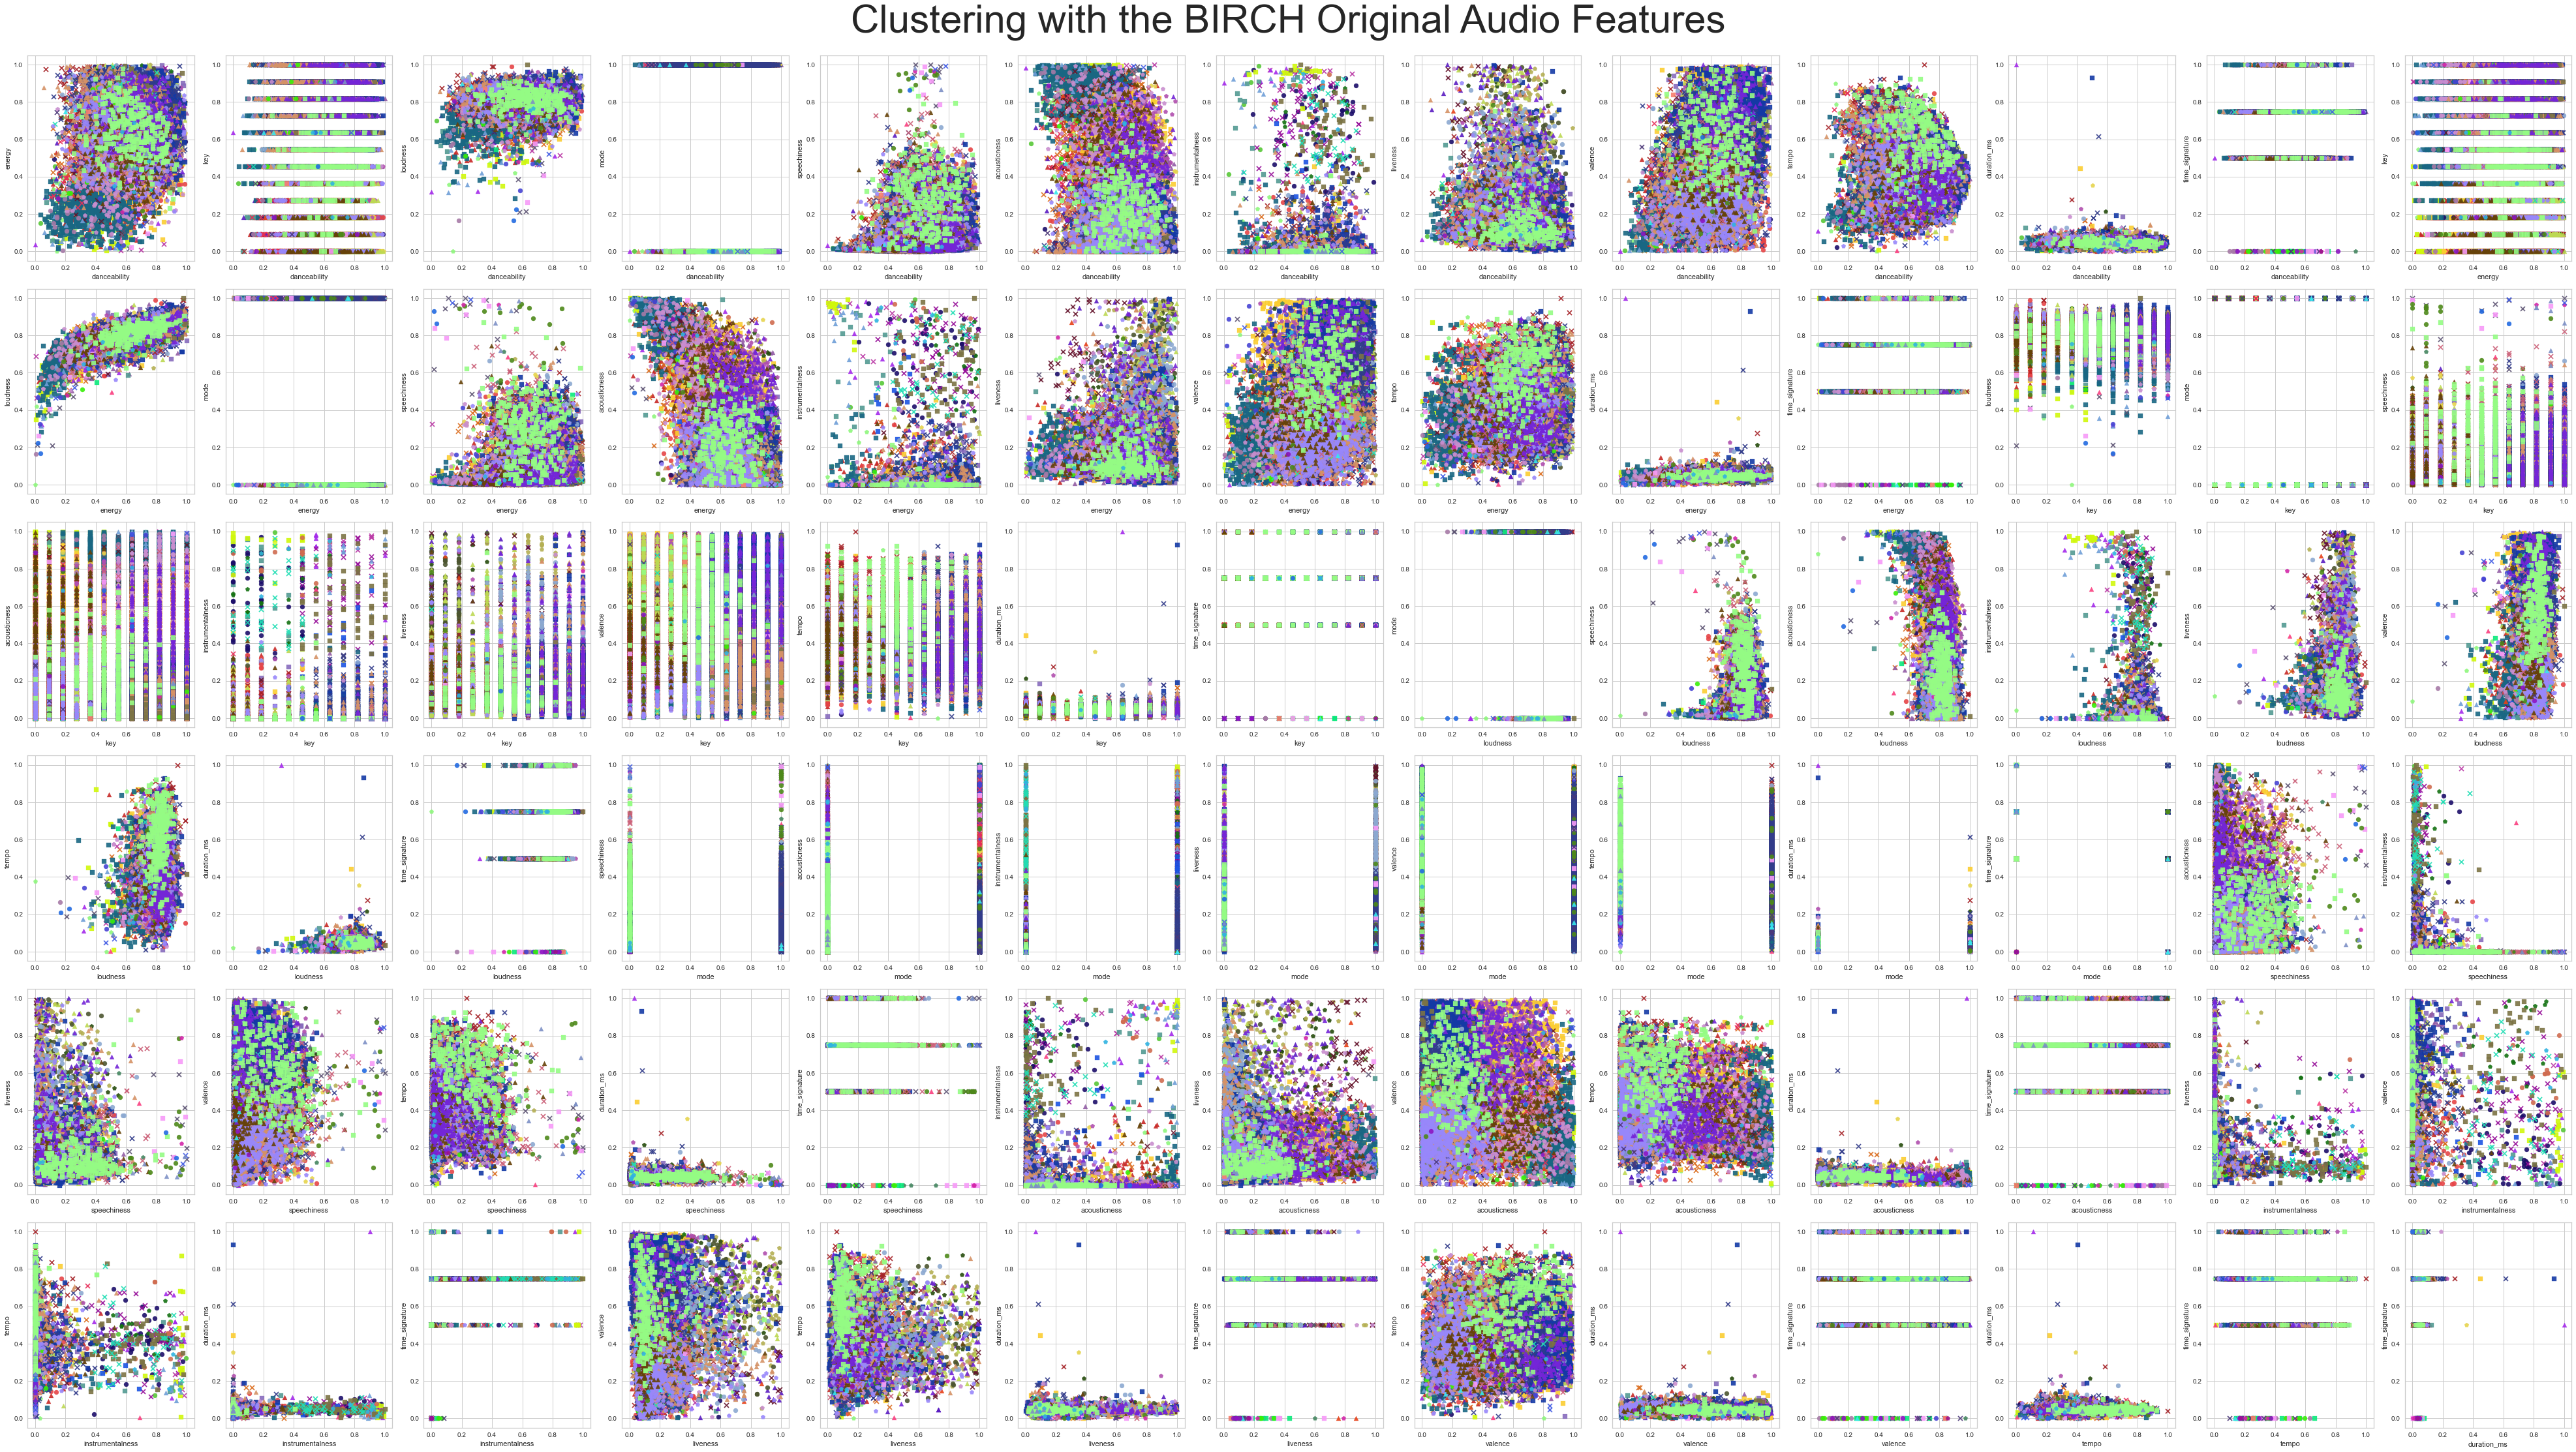
\includegraphics[scale=0.07]{Outputs/BIRCH Clustering - Original Audio Features.png}
    \caption{BIRCH clustering on the scaled original audio features}
    \label{fig:birch-first}
\end{figure}
\begin{figure}[!htb]
    \centering
    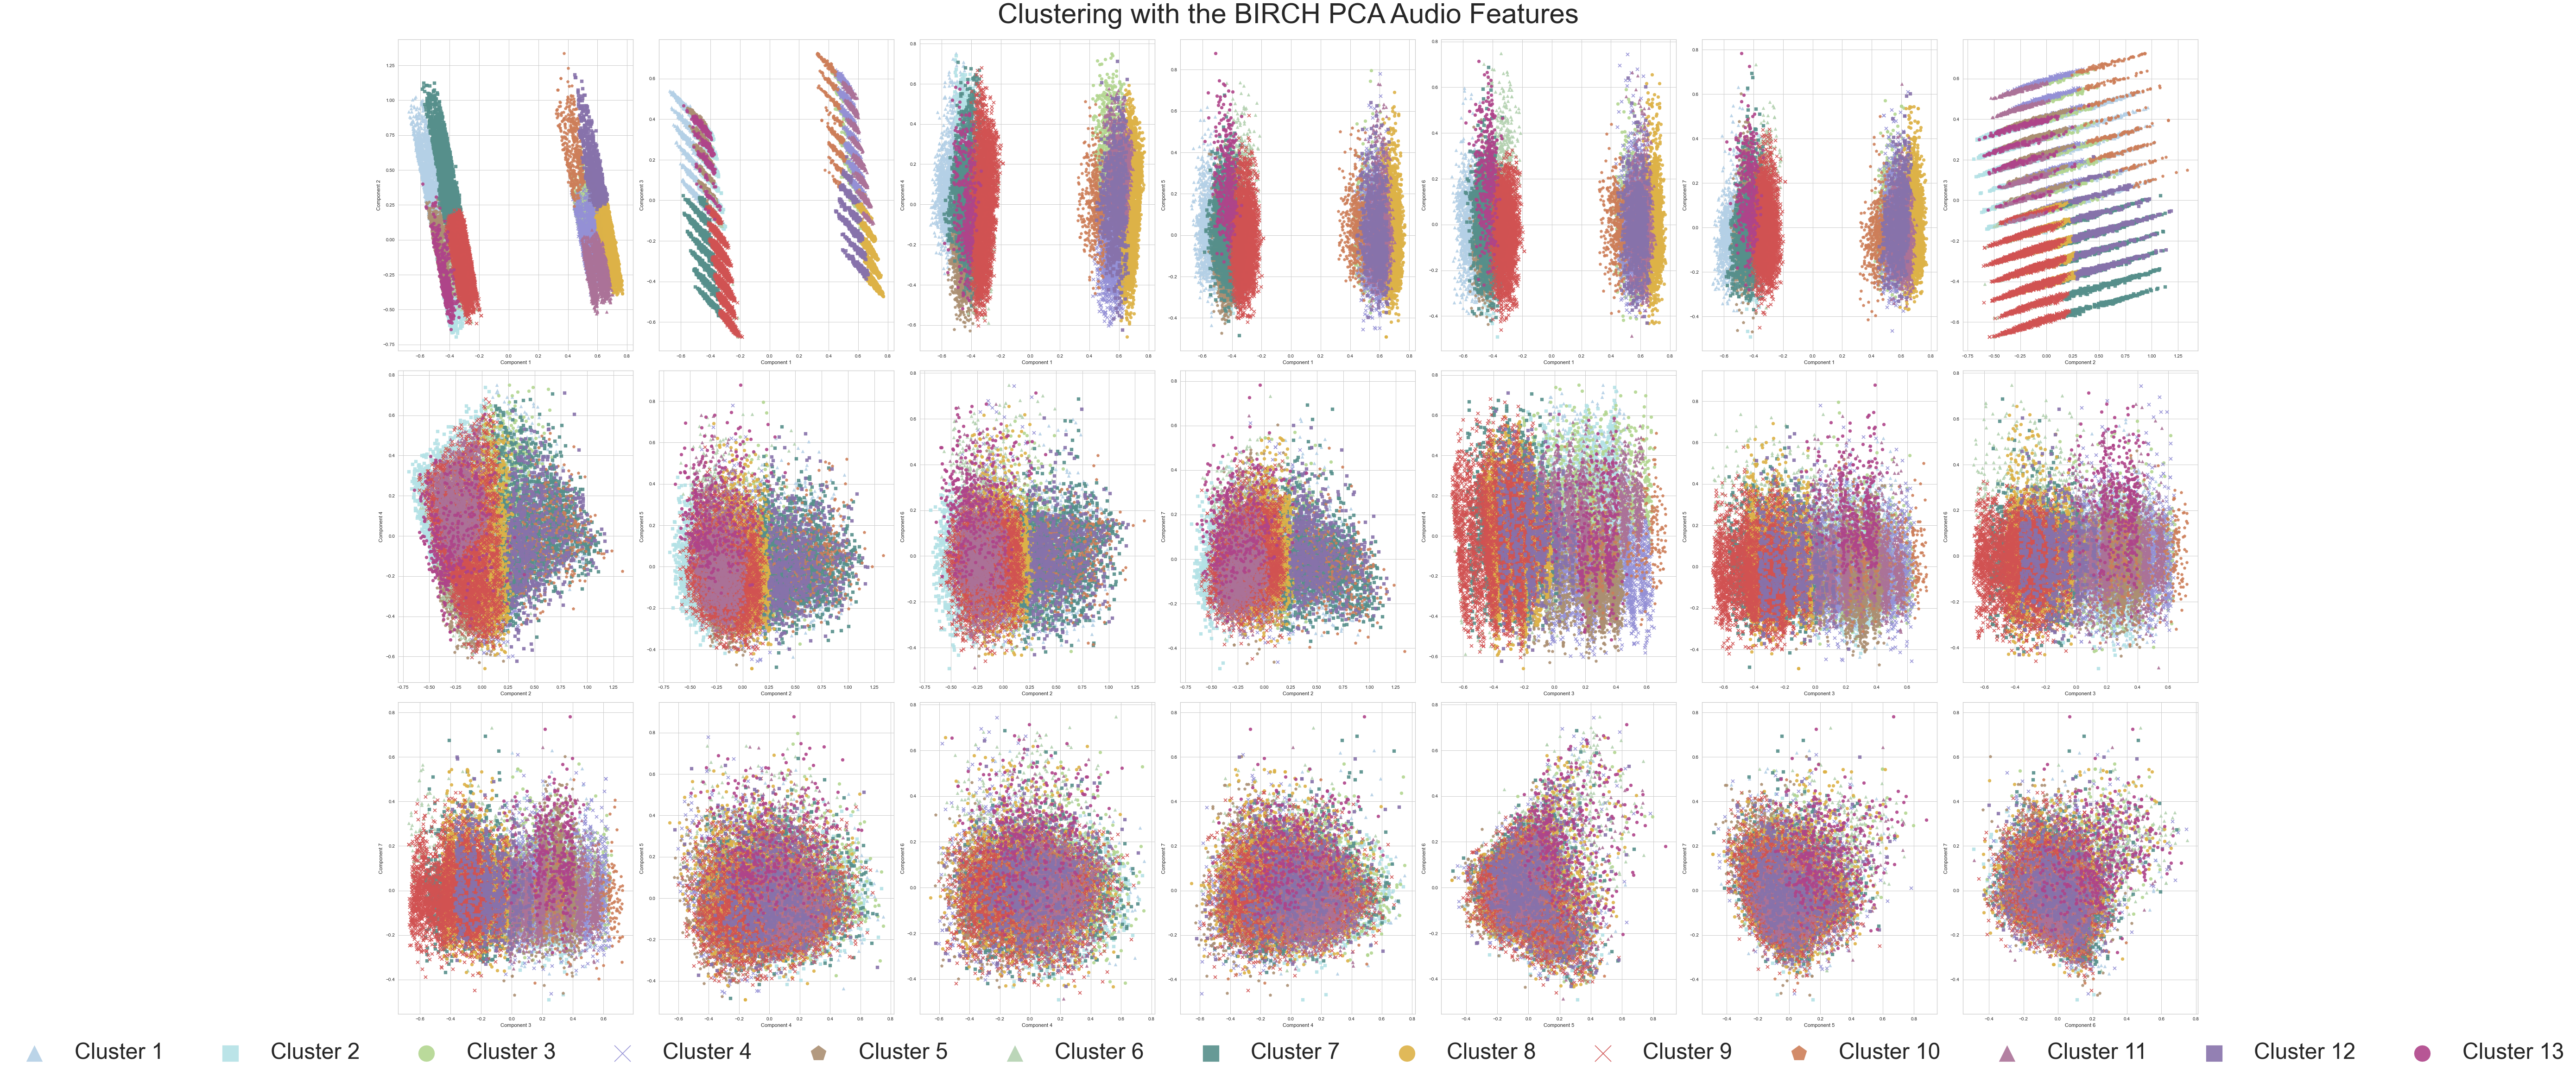
\includegraphics[scale=0.07]{Outputs/BIRCH Clustering - PCA Audio Features.png}
    \caption{BIRCH clustering on PCA dervived audio features}
    \label{fig:birch-second}
\end{figure}
\begin{figure}[!htb]
    \centering
    \includegraphics[scale=0.08]{Outputs/BIRCH Clustering - UMAP Audio Features.png}
    \caption{BIRCH clustering on UMAP derived audio features}
    \label{fig:birch-third}
\end{figure}
\begin{figure}[!htb]
    \centering
    \includegraphics[scale=0.08]{Outputs/BIRCH Clustering - Gaussian Random Projections Audio Features.png}
    \caption{BIRCH clustering on Gaussian Random Projections derived audio features}
    \label{fig:birch-fourth}
\end{figure}
\begin{figure}[htp]
    \centering
    \includegraphics[scale=0.08]{Outputs/BIRCH Clustering - PaCMAP Audio Features.png}
    \caption{BIRCH clustering on the PaCMAP derived audio features}
    \label{fig:birch-fifth}
\end{figure}
\begin{figure}[htp]
    \centering
    \includegraphics[scale=0.08]{Outputs/BIRCH Clustering - Autoencoder Audio Features.png}
    \caption{BIRCH clustering on the Autoencoder derived audio features}
    \label{fig:birch-sixth}
\end{figure}
\FloatBarrier
\subsection{DBSCAN}
\begin{figure}[htp]
    \centering
    \includegraphics[scale=0.09]{Outputs/DBSCAN Clustering - Original Audio Features.png}
    \caption{DBSCAN clustering on the scaled original audio features}
    \label{fig:dbscan-first}
\end{figure}
\begin{figure}[!htb]
    \centering
    \includegraphics[scale=0.09]{Outputs/DBSCAN Clustering - PCA Audio Features.png}
    \caption{DBSCAN clustering on PCA dervived audio features}
    \label{fig:dbscan-second}
\end{figure}
\begin{figure}
    \centering
    \includegraphics[scale=0.08]{Outputs/DBSCAN Clustering - UMAP Audio Features.png}
    \caption{DBSCAN clustering on UMAP derived audio features}
    \label{fig:dbscan-third}
\end{figure}
\begin{figure}
    \centering
    \includegraphics[scale=0.08]{Outputs/DBSCAN Clustering - Gaussian Random Projections Audio Features.png}
    \caption{DBSCAN clustering on Gaussian Random Projections derived audio features}
    \label{fig:dbscan-fourth}
\end{figure}
\begin{figure}
    \centering
    \includegraphics[scale=0.09]{Outputs/DBSCAN Clustering - PaCMAP Audio Features.png}
    \caption{DBSCAN clustering on the PaCMAP derived audio features}
    \label{fig:dbscan-fifth}
\end{figure}
\begin{figure}
    \centering
    \includegraphics[scale=0.09]{Outputs/DBSCAN Clustering - Autoencoder Audio Features.png}
    \caption{DBSCAN clustering on the Autoencoder derived audio features}
    \label{fig:dbscan-sixth}
\end{figure}
\FloatBarrier
\section{K-Means with PaCMAP Cluster Analysis}
\label{appendix:D}
Some observations from the grid plot reveal that cluster 5 has songs with highest danceability, energy, loudness, valence and tempos while those in cluster 2 are more melodious (as characterised by their low energy and danceability and high acousticness). While the songs in cluster 0 and 1 also contain some rave tracks, the difference lies in their keys, speechiness and skewness of the valence attributes. Cluster 7 is a sparse cluster which contains songs with high instrumentalness.
\begin{figure}[!htb]
    \centering
    \includegraphics[scale=0.6]{Outputs/Best Algorithm Cluster Analysis.pdf}
    \caption{K-Means with PaCMAP cluster representations in terms of the 13 audio features}
    \label{fig:kmeans-pacmap}
\end{figure}
\clearpage
\section{Artist Clustering}
\label{appendix:E}
\begin{table}[h]
\centering
\begin{tabular}{|l|r|r|r|r|r|r|r|r|r|}
\toprule
{Artist} &    0 &    1 &    2 &    3 &    4 &    5 &    6 &    7 &    8 \\
\midrule
Denki Groove              &  0.0 &  0.0 &  1.0 &  0.0 &  2.0 &  0.0 &  0.0 &  0.0 &  1.0 \\
Marshmello                &  1.0 &  1.0 &  3.0 &  0.0 &  0.0 &  0.0 &  1.0 &  0.0 &  1.0 \\
Rafet El Roman            &  0.0 &  0.0 &  0.0 &  0.0 &  0.0 &  0.0 &  0.0 &  1.0 &  0.0 \\
Katncandix2               &  0.0 &  0.0 &  0.0 &  1.0 &  0.0 &  0.0 &  0.0 &  0.0 &  1.0 \\
Ikke Hüftgold             &  0.0 &  0.0 &  0.0 &  0.0 &  0.0 &  0.0 &  1.0 &  0.0 &  0.0 \\
Beverly                   &  0.0 &  0.0 &  2.0 &  0.0 &  0.0 &  0.0 &  0.0 &  0.0 &  0.0 \\
Kim Churchill             &  1.0 &  0.0 &  0.0 &  0.0 &  0.0 &  0.0 &  0.0 &  0.0 &  0.0 \\
Tim Arisu                 &  0.0 &  0.0 &  1.0 &  0.0 &  0.0 &  0.0 &  0.0 &  0.0 &  0.0 \\
Pitbull                   &  3.0 &  1.0 &  7.0 &  0.0 &  0.0 &  2.0 &  5.0 &  1.0 &  0.0 \\
Savage Garden             &  0.0 &  0.0 &  1.0 &  0.0 &  0.0 &  0.0 &  0.0 &  0.0 &  0.0 \\
Hornet La Frappe          &  0.0 &  7.0 &  2.0 &  0.0 &  5.0 &  0.0 &  1.0 &  7.0 &  0.0 \\
Dengaz                    &  0.0 &  1.0 &  0.0 &  0.0 &  1.0 &  0.0 &  0.0 &  0.0 &  0.0 \\
Snakehips                 &  0.0 &  0.0 &  2.0 &  0.0 &  0.0 &  0.0 &  1.0 &  0.0 &  0.0 \\
Kyle Edwards;Chris Bevrly &  0.0 &  1.0 &  0.0 &  0.0 &  0.0 &  0.0 &  0.0 &  0.0 &  0.0 \\
Andra Day                 &  0.0 &  0.0 &  0.0 &  2.0 &  0.0 &  0.0 &  0.0 &  0.0 &  0.0 \\
IKE                       &  0.0 &  0.0 &  1.0 &  0.0 &  0.0 &  0.0 &  0.0 &  0.0 &  0.0 \\
EXO                   &  2.0 &  1.0 &   6.0 &  2.0 &  4.0 &   1.0 &  3.0 &  2.0 &  3.0 \\
Crowded House             &  0.0 &  1.0 &  0.0 &  0.0 &  0.0 &  0.0 &  0.0 &  0.0 &  0.0 \\
Mitch James               &  0.0 &  0.0 &  0.0 &  1.0 &  0.0 &  1.0 &  0.0 &  0.0 &  0.0 \\
La Combo Tortuga          &  0.0 &  0.0 &  1.0 &  0.0 &  0.0 &  1.0 &  2.0 &  0.0 &  0.0 \\
Alex Rose                 &  0.0 &  0.0 &  0.0 &  0.0 &  1.0 &  0.0 &  0.0 &  0.0 &  0.0 \\
100\%                      &  0.0 &  0.0 &  0.0 &  0.0 &  0.0 &  0.0 &  0.0 &  1.0 &  0.0 \\
MFÖ                       &  1.0 &  0.0 &  0.0 &  0.0 &  0.0 &  0.0 &  0.0 &  0.0 &  0.0 \\
Marianas Trench           &  0.0 &  0.0 &  1.0 &  0.0 &  0.0 &  0.0 &  0.0 &  0.0 &  0.0 \\
Joshua Garcia             &  0.0 &  1.0 &  0.0 &  0.0 &  0.0 &  0.0 &  0.0 &  0.0 &  0.0 \\
Leonardo Lamacchia        &  0.0 &  1.0 &  0.0 &  0.0 &  0.0 &  0.0 &  0.0 &  0.0 &  0.0 \\
Natalie Imbruglia         &  0.0 &  0.0 &  0.0 &  0.0 &  0.0 &  0.0 &  1.0 &  0.0 &  0.0 \\
Crecer German             &  0.0 &  0.0 &  0.0 &  0.0 &  1.0 &  0.0 &  0.0 &  0.0 &  0.0 \\
The xx                    &  0.0 &  1.0 &  0.0 &  4.0 &  5.0 &  0.0 &  1.0 &  1.0 &  3.0 \\
Urban Cone                &  0.0 &  0.0 &  1.0 &  0.0 &  0.0 &  0.0 &  1.0 &  0.0 &  0.0 \\
\bottomrule
\end{tabular}
\end{table}
\section{Clustering using Trends}
\label{appendix:F}
\subsection{Introduction}
The idea here was to cluster songs with a similar trajectories as shown in figure \label{fig:trendstwosongs}. To cluster them by simply feeding in the steaming data for the whole year would make the number of features too high for the clustering model. We used two ways to capture the mathematical information about the trends which were - using the features from the encoder layer of a convolution autoencoder and the transformed features from polynomial regression. 

\begin{figure}[h]
\centering
\centerline{\includegraphics[scale=0.6]{Outputs/cluster example 1.png}}
\caption{Trends of two similar songs}
\label{fig:trendstwosongs}
\end{figure}

\subsection{Data Preparation}
We selected the songs in the global region as they had most number of streams as shown in \label{fig:streamsper}. We used the song's URL as keys for each song, as many songs have the name track name.

\begin{figure}[h]
\centering
\centerline{\includegraphics[width=\textwidth]{Outputs/streams per region.png}}
\caption{Barplot of regions with their total streams throughout the year}
\label{fig:streamsper}
\end{figure}

For each song, we fetched the total number of streams and normalised them to the range of [0,1]. We then 0 padded the array for the days the songs were not present in the charts.

\subsection{Methods}
\textbf{Convolutional Autoencoder} - humans use visual features to compare trends - features like shapes and slopes. Convolution Neural Networks work exceptionally well on image classification tasks and just like humans as they can capture visual features like edges and shapes accurately. Using a convolutional autoencoder with the encoded images as features could capture the visual features for the trends of songs.

We converted the streams of each song into trends as images of size 28x28. This image was fed into the convolutional autoencoder and after training, the encoded information of each image were reconstructed. We used the features from the encoder layer for clustering using K-Means. 

\textbf{Polynomial Regression} -
To capture the mathematical features of a trend one can fit a curve to it and use the parameters of the curve as features to define the curve.

For the normalised streams of each song we fit a ploynomial regressor with 5 parameters. There 5 parameters/coefficients were stored and then fed to the K-Means clustering algorithm as its features.

\subsection{Results and Conclusion}
The convolutional autoencoder-based clustering didn't work well as it was just resizing the image and not learning the edges, shapes or any of the other mathematical features from the curves (see \ref{fig:caout}). Also, the encoded features were still in 2 dimensions, so these features lost the relationships to its nearby pixels when flattened, and the number of features were still too high for the clustering algorithm to work with.

\begin{figure}[h]
\centering
\centerline{\includegraphics[width=\textwidth]{Outputs/caout.png}}
\caption{Output of the trends from the encoder layer}
\label{fig:caout}
\end{figure}
The polynomial feature-based clustering was able to cluster similar trends together as shown in \label{fig:polyout} . But, it could not cluster similar trends for songs which lasted on the charts for different number of days. The results are tabluated in \ref{tab:table4}

For this to work, we would need the complete data, i.e. all the songs, should have data for each day of the year. Or if we have labels for the cluster, i.e. if we could train in a supervised manner, then a classification algorithm will be able to match songs with similar trends irrespective of the days that it lasts on the charts.
\begin{figure}[h]
\centering
\centerline{\includegraphics[width=\textwidth]{Outputs/resultploy.png}}
\caption{Trends and their cluster labels after polynomial regressor based clustering with K-Means}
\label{fig:polyout}
\end{figure}

\begin{table}[!hbt]
    \centering
    \rowcolors{1}{white}{gray!25}
    \resizebox{\columnwidth}{!}{%
    \begin{tabular}{|c|c|c|c|c|c|c|}
    \toprule
     \makecell{Clustering \\ Algorithm} & \makecell{Feature Engineering}  & \makecell{No. Clusters} & \makecell{No. Features} & 
     \makecell{CH} & \makecell{DB} & \makecell{SS} \\
    \midrule
        K-Means  & Convolutional Autoencoder      &  12      & 49    & 377.00    & 1.381  & 0.401\\
        K-Means  &  Polynomial Regressor     &  20     & 5     & 6427.71    & 0.748   & 0.527\\
    \bottomrule
    \end{tabular}%
    }
    \caption{Experiment results for the two feature engineering methods with K-Means. SS is silhouette score, DB is Davies–Bouldin index, CH is Calinski Harabasz score.}
    \label{tab:table4}
\end{table} 
\end{appendix}